\documentclass[10pt]{beamer}

\usetheme[progressbar=frametitle]{metropolis}

\usepackage{booktabs}
\usepackage[scale=2]{ccicons}


\usepackage{amsmath}
\usepackage{pgfplots}
\usepgfplotslibrary{dateplot}

\usepackage{xspace}
\newcommand{\themename}{\textbf{\textsc{metropolis}}\xspace}

%\usepackage{placeins} %%%
\usepackage{subfig}
\usepackage{physics}
\usepackage{amssymb}


\usepackage{tikz}
\usepackage{circuitikz}
\usepackage{siunitx}


\usepackage{latexsym}
\usepackage{mathtools}
\usepackage{slashed} % for the Feynman slash notation

\usepackage{listings}

\usepackage{balance}


% edited by Mauro 28-12-16
%
%% <local definitions>
\newcommand{\R}{\mathbb{R}}	
\newcommand{\C}{\mathbb{C}}
\newcommand{\HQ}{\mathbb{H}}
\newcommand{\N}{\mathbb{N}}
\newcommand{\be}{\begin{equation}}
\newcommand{\ee}{\end{equation}}	
\newcommand{\bea}{\begin{eqnarray}}
\newcommand{\eea}{\end{eqnarray}}	
\newcommand{\Pin}{\mathrm{Pin}}	
\newcommand{\Spin}{\mathrm{Spin}}
\renewcommand{\O}{\mathrm{O}}
\newcommand{\SO}{\mathrm{SO}}
\renewcommand{\eqref}[1]{(\ref{#1})}
\newcommand{\cl}[1]{\ensuremath{Cl(#1)}} % #1 stands for the values p,q. $\cl{p,q}$ produces 'Cl(p,q)'.
\newcommand{\gvec}[1]{\ensuremath{\mbox{\textbf{\textit{#1}}}}}
\newcommand{\vect}[1]{\ensuremath{\mbox{\textbf{\textit{#1}}}}}
%% </local definitions>

\newcommand{\Ba}[0]{\mathbf{a}}
\newcommand{\Bb}[0]{\mathbf{b}}
\newcommand{\Bc}[0]{\mathbf{c}}
\newcommand{\Bd}[0]{\mathbf{d}}
\newcommand{\Be}[0]{\mathbf{e}}
\newcommand{\Bf}[0]{\mathbf{f}}
\newcommand{\Bg}[0]{\mathbf{g}}
\newcommand{\Bh}[0]{\mathbf{h}}
\newcommand{\Bi}[0]{\mathbf{i}}
\newcommand{\Bj}[0]{\mathbf{j}}
\newcommand{\Bk}[0]{\mathbf{k}}
\newcommand{\Bl}[0]{\mathbf{l}}
\newcommand{\Bm}[0]{\mathbf{m}}
\newcommand{\Bn}[0]{\mathbf{n}}
\newcommand{\Bo}[0]{\mathbf{o}}
\newcommand{\Bp}[0]{\mathbf{p}}
\newcommand{\Bq}[0]{\mathbf{q}}
\newcommand{\Br}[0]{\mathbf{r}}
\newcommand{\Bs}[0]{\mathbf{s}}
\newcommand{\Bt}[0]{\mathbf{t}}
\newcommand{\Bu}[0]{\mathbf{u}}
\newcommand{\Bv}[0]{\mathbf{v}}
\newcommand{\Bw}[0]{\mathbf{w}}
\newcommand{\Bx}[0]{\mathbf{x}}
\newcommand{\By}[0]{\mathbf{y}}
\newcommand{\Bz}[0]{\mathbf{z}}
\newcommand{\BA}[0]{\mathbf{A}}
\newcommand{\BB}[0]{\mathbf{B}}
\newcommand{\BC}[0]{\mathbf{C}}
\newcommand{\BD}[0]{\mathbf{D}}
\newcommand{\BE}[0]{\mathbf{E}}
\newcommand{\BF}[0]{\mathbf{F}}
\newcommand{\BG}[0]{\mathbf{G}}
\newcommand{\BH}[0]{\mathbf{H}}
\newcommand{\BI}[0]{\mathbf{I}}
\newcommand{\BJ}[0]{\mathbf{J}}
\newcommand{\BK}[0]{\mathbf{K}}
\newcommand{\BL}[0]{\mathbf{L}}
\newcommand{\BM}[0]{\mathbf{M}}
\newcommand{\BN}[0]{\mathbf{N}}
\newcommand{\BO}[0]{\mathbf{O}}
\newcommand{\BP}[0]{\mathbf{P}}
\newcommand{\BQ}[0]{\mathbf{Q}}
\newcommand{\BR}[0]{\mathbf{R}}
\newcommand{\BS}[0]{\mathbf{S}}
\newcommand{\BT}[0]{\mathbf{T}}
\newcommand{\BU}[0]{\mathbf{U}}
\newcommand{\BV}[0]{\mathbf{V}}
\newcommand{\BW}[0]{\mathbf{W}}
\newcommand{\BX}[0]{\mathbf{X}}
\newcommand{\BY}[0]{\mathbf{Y}}
\newcommand{\BZ}[0]{\mathbf{Z}}

\newcommand{\ta}[0]{\tilde{a}}
\newcommand{\tb}[0]{\tilde{b}}
\newcommand{\tc}[0]{\tilde{c}}
\newcommand{\td}[0]{\tilde{d}}

\newcommand{\hA}[0]{\hat{A}}
\newcommand{\hB}[0]{\hat{B}}
\newcommand{\hH}[0]{\hat{H}}

\newcommand{\tA}[0]{\tilde{A}}
\newcommand{\tF}[0]{\tilde{F}}
\newcommand{\tE}[0]{\tilde{E}}
\newcommand{\tH}[0]{\tilde{H}}
\newcommand{\tJ}[0]{\tilde{J}}

% spinors definition
\newcommand{\barJ}[0]{\bar{J}}
\newcommand{\barF}[0]{\bar{F}}
\newcommand{\barP}[0]{\bar{P}}
\newcommand{\barW}[0]{\bar{W}}



\newcommand{\tnabla}[0]{\tilde{\nabla}}
\newcommand{\tphi}[0]{\tilde{\phi}}
\newcommand{\tpsi}[0]{\tilde{\psi}}

%
\newcommand{\wavep}[0]{\partial^+}
\newcommand{\wavem}[0]{\partial^-}

\newcommand{\wavepp}[0]{\tilde{\partial}^+}
\newcommand{\wavemp}[0]{\tilde{\partial}^-}

\newcommand{\wavepd}[0]{\bar{\partial}^+}
\newcommand{\wavemd}[0]{\bar{\partial}^-}

\newcommand{\pbd}[0]{\bar{\partial}_d}

% frequency

\newcommand{\helmp}[0]{{\underline{\partial}}^+}
\newcommand{\helmm}[0]{{\underline{\partial}}^-}

\newcommand{\helmpp}[0]{{\underline{\tilde{\partial}}}^+}
\newcommand{\helmmp}[0]{{\underline{\tilde{\partial}}}^-}

\newcommand{\helmpd}[0]{{\underline{\bar{\partial}}}^+}
\newcommand{\helmmd}[0]{{\underline{\bar{\partial}}}^-}

\newcommand{\pbfd}[0]{{\underline{\bar{\partial}}}_d}




\def \figname {Figure}
\def \emode {E }
\def \hmode {H }
\def \temode {TE }
\def \tmmode {TM }
\def \temoden {TE${}_n$ }
\def \tmmoden {TM${}_n$ }
\def \temodemn {TE${}_{mn}$ }
\def \tmmodemn {TM${}_{mn}$ }



\newcommand{\iGA}{{i}}
\newcommand{\conjg}[1] {\ensuremath{#1}^*}

\setbeamertemplate{bibliography item}{[\theenumiv]}


\title{Linearity and Superposition}

\date{}

%\subtitle{Maximizing efficiency and power at a fixed frequency}
%\date{\today}
%\author{Alessandra Costanzo, Franco Mastri, Mauro Mongiardo*, Giuseppina Monti}
%\institute{*Department of Engineering,
%University of Perugia, Italy}

\author{ Mauro Mongiardo$^1$}

\institute{ $^1$ Department of Engineering, University of Perugia, Perugia, Italy.
}

%
\titlegraphic{\hfill
\includegraphics[height=1.5cm]{logo}}


\begin{document}

\maketitle

\begin{frame}{Table of contents}
  \setbeamertemplate{section in toc}[sections numbered]
  \tableofcontents[hideallsubsections]
\end{frame}


%=========================================================================
\begin{frame}[shrink=40]{Physical Constants}


%\chapter*{\center Physical Constants}
%\typeout{Physical Constants}
%\addcontentsline{toc}{chapter}{Physical Constants}
\begin{center}
\begin{tabular}{||l|lll||} 
\hline
{\bf Name}&{\bf Symbol}&{\bf Value}&{\bf Unit}\\
\hline
\hline
Number $\pi$                 &$\pi$&3.14159265358979323846&\\
Number e                     &e    &2.71828182845904523536&\\
Euler's constant &\multicolumn{3}{|l||}{$\gamma=\lim\limits_{n\rightarrow\infty}\left(\sum\limits_{k=1}^n 1/k-\ln(n)\right)=0.5772156649$}\\
\hline
Elementary charge            &$e$&$1.60217733\cdot10^{-19}$&C\rule{0pt}{13pt}\\
Gravitational constant       &$G,\kappa$&$6.67259\cdot10^{-11}$&m$^3$kg$^{-1}$s$^{-2}$\\
%Fine-structure constant      &$\alpha=e^2/2hc\varepsilon_0$&$\approx1/137$&\\
Speed of light in vacuum     &$c$&$2.99792458\cdot10^8$&m/s (def)\\
Permittivity of the vacuum   &$\varepsilon_0$&$8.854187\cdot10^{-12}$&F/m\\
Permeability of the vacuum   &$\mu_0$&$4\pi\cdot10^{-7}$&H/m\\
%$(4\pi\varepsilon_0)^{-1}$   &&$8.9876\cdot10^9$&Nm$^2$C$^{-2}$\\
\hline
%Planck's constant            &$h$&$6.6260755\cdot10^{-34}$&Js\rule{0pt}{13pt}\\
%Dirac's constant             &$\hbar=h/2\pi$&$1.0545727\cdot10^{-34}$&Js\\
%Bohr magneton                &$\mu_{\rm B}=e\hbar/2m_{\rm e}$&$9.2741\cdot10^{-24}$&Am$^2$\\
%Bohr radius                  &$a_0$&$0.52918$&\AA\\
%Rydberg's constant           &$Ry$&13.595&eV\\
%Electron Compton wavelength  &$\lambda_{\rm Ce}=h/\me c$&$2.2463\cdot10^{-12}$&m\\
%Proton Compton wavelength    &$\lambda_{\rm Cp}=h/m_{\rm p}c$&$1.3214\cdot10^{-15}$&m\\
%Reduced mass of the H-atom   &$\mu_{\rm H}$&$9.1045755\cdot10^{-31}$&kg\\
%\hline
%Stefan-Boltzmann's constant  &$\sigma$&$5.67032\cdot10^{-8}$&Wm$^{-2}$K$^{-4}$\rule{0pt}{13pt}\\
%Wien's constant              &$k_{\rm W}$&$2.8978\cdot10^{-3}$&mK\\
%\hline
%Molar gasconstant            &$R$&8.31441&J$\cdot$mol$^{-1}\cdot$K$^{-1}$\\
%Avogadro's constant          &$N_{\rm A}$&$6.0221367\cdot10^{23}$&mol$^{-1}$\\
%Boltzmann's constant         &$k=R/N_{\rm A}$&$1.380658\cdot10^{-23}$&J/K\\
\hline
Electron mass                &$m_{\rm e}$&$9.1093897\cdot10^{-31}$&kg\rule{0pt}{13pt}\\
Proton mass                  &$m_{\rm p}$&$1.6726231\cdot10^{-27}$&kg\\
Neutron mass                 &$m_{\rm n}$&$1.674954\cdot10^{-27}$&kg\\
%Elementary mass unit         &$m_{\rm u}=\frac{1}{12}m(^{12}_{~6}$C)&$1.6605656\cdot10^{-27}$&kg\\
%Nuclear magneton             &$\mu_{\rm N}$&$5.0508\cdot10^{-27}$&J/T\\
\hline
Diameter of the Sun          &$D_\odot$&$1392\cdot10^6$&m\rule{0pt}{13pt}\\
Mass of the Sun              &$M_\odot$&$1.989\cdot10^{30}$&kg\\
Rotational period of the Sun &$T_\odot$&25.38&days\\
Radius of Earth              &$R_{\rm A}$&$6.378\cdot10^6$&m\\
Mass of Earth                &$M_{\rm A}$&$5.976\cdot10^{24}$&kg\\
Rotational period of Earth   &$T_{\rm A}$&23.96&hours\\
Earth orbital period         &Tropical year&365.24219879&days\\
Astronomical unit            &AU&$1.4959787066\cdot10^{11}$&m\\
Light year                   &lj&$9.4605\cdot10^{15}$&m\\
%Parsec                       &pc&$3.0857\cdot10^{16}$&m\\
%Hubble constant              &$H$&$\approx(75\pm25)$&km$\cdot$s$^{-1}\cdot$Mpc$^{-1}$\\
\hline
\end{tabular}
\label{PhysicalConstants}
\end{center}


\end{frame}



%=========================================================================
\section{Coulomb's law}
%=========================================================================
%=========================================================================
\begin{frame}[fragile]{Coulomb's law}
%\subsection{Coulomb's law}
%
Two charged points with \alert{charges of the same sign are repulsing},
while points with \alert{charges of opposite signs are attracting} with
force proportional to quantities of their charges and inverse
proportional to square of distance between them:
\be
F = k \frac{Q_1\,Q_2}{r^2}. \label{coulomb}
%\tag1.1
\ee
with 
\be
k = \frac{1}{4 \pi \epsilon_0} = \frac{c^2\mu_0}{4 \pi }.
\ee

\end{frame}
%=========================================================================

\begin{frame}[fragile]{Coulomb's law}

\begin{figure}
\centering
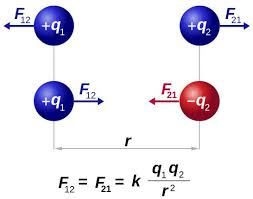
\includegraphics[width=40mm]{Coulomb.jpeg}
\caption{Figure illustrating the Force between two electrical charges }
\label{echarges}
\end{figure}

\end{frame}


%=========================================================================
\begin{frame}[fragile]{}

Force $F$ defined by the relationship (\ref{coulomb}) is \alert{strong}.

However, in everyday life it does not reveal itself. 
This is due
to the \alert{{\it screening}}. 

\alert{The numbers of positive and negative charges
in nature are exactly balanced}. Atoms and molecules, which
constitute all observable matter around us, have the same amount of
positive and negative charges. 

Therefore they are electrically neutral
in whole. 

%Force (\ref{coulomb}) reveals itself in form of chemical links only when atoms are pulled together.
\end{frame}

%=========================================================================
\section{Currents}
%=========================================================================
\begin{frame}[fragile]{Currents}
Electric current arises as a result of \alert{motion of charged points}.

This occurs in metallic conductor, which usually have lengthy form
(form of wire). Current in such conductor is determined by the
\alert{{\it amount of charge passing through it within the unit of
time}}. 
%Therefore for unit of current we have:
%\be
%%\gather
%\text{\it unit of current in SGS}
%=\text{\it unit of charge in SGS $\cdot$ sec$^{-1}$}=\\
%=\text{\it g$^{\,1\!/2}$ $\cdot$ cm$^{\,3/2}$ $\cdot$ sec$^{-2}$}.
%%\endgather
%\ee

Let's consider straight conducting rod of the length $l$. 

Current
in it leads to \alert{misbalance of charges in its ends}. Charges of
definite sign move to one end of the rod, while lack of these
charges in the other end of the rod is detected as the charge
of opposite sign. 

Then Coulomb force  arises that
tends to recover balance of charges in electrically neutral
rod. 

This means that in such rod \alert{current could not flow in
constant direction during long time}. 

\end{frame}

%=========================================================================
\begin{frame}[fragile]{Circular ring}
Another situation when we consider
a conductor of the form of ring or circuit. 

Here current
does not break the balance of charges. 

Direct current can flow
in it during unlimitedly long time. 

Circular conductor itself
thereby remains electrically neutral and no Coulomb forces
arise.
%\par
%\parshape 11 0cm 10.1cm 0cm 10.1cm 0cm 10.1cm 0cm 10.1cm
%0cm 10.1cm 0cm 10.1cm 0cm 10.1cm 0cm 10.1cm 0cm 10.1cm
%5cm 5.1cm 5cm 5.1cm

 In spite of absence of Coulomb forces, in experiments
\alert{the interaction of two circular conductors with currents has been
detected}. 

This interaction has other nature, it is not due 
to electrical, but due to \alert{magnetic forces}. 


\end{frame}
%=========================================================================
\begin{frame}[fragile]{}
\begin{figure}
\centering
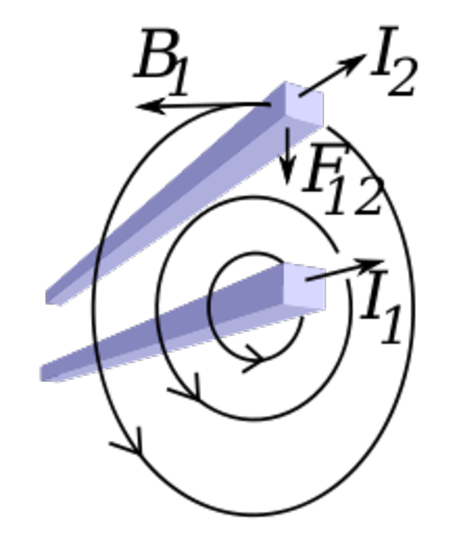
\includegraphics[width=30mm]{FigAmpere.pdf}
\caption{Force between two filaments with currents }
\label{echarges}
\end{figure}


\end{frame}

%=========================================================================
\begin{frame}[fragile]{}
The \alert{magnitude
of magnetic forces depends essentially on the shape and
mutual arrangement} of circular conductors. 

In order to reveal
quantitative characteristics for magnetic forces it is convenient to simplify the geometry of conductors. To this end,
they are deformed so that each possesses straight rod-shaped
part of sufficiently large length $l$. 

These rod--shaped parts are
arranged parallel to each other with the distance $r$ between
them.

 In the limit, when $l$ is much larger than $r$, this
configuration of conductors can be treated as \alert{a pair of infinitely
long parallel conductors}.

\end{frame}
%=========================================================================
\section{Ampere Law}
%=========================================================================

\begin{frame}[fragile]{Amper Law}
In experiments it was found that such conductors do
interact according to the following law.
%\subsection{ Ampere law}
%\parshape 4 5cm 5.1cm 5cm 5.1cm 5cm 5.1cm 0cm 10.1cm

\alert{Force of interaction of  two  infinite 
parallel conductors with currents per unit length of them is proportional
to the values of currents in them and inverse proportional to the distance
between them}:
\be
\frac{F}{l} = 2 k_A\frac{I_1\,I_2}{r}. \label{quasiAmpere}
%\tag1.3
\ee
with
\be
k_A = \frac{\mu_0}{4 \pi}
\ee
Two co-directed currents attract each other, while opposite directed
currents repulse each other.

What is $\mu_0$?
\end{frame}

%=========================================================================
\begin{frame}[fragile]{}
\alert{In SI measure unit of current \SI{1}{\ampere} (one {\it ampere}) is a fundamental
unit}. 

It is determined such that we have
\be
\frac{F}{l}=\frac{2\,\mu_0}{4\pi}\frac{I_1\,I_2}{r}. \label{AAAmpere}
%\tag1.6
\ee

Here $\pi=3.14\dots$ is exact (though it is irrational) mathematical
constant with no measure unit. 

\alert{Constant $\mu_0$ is called {\it magnetic
permeability} of vacuum}. It has the (conventional) measure unit reported in Table \ref{PhysicalConstants}
%\be
%\mu_0=4\pi\cdot 10^{-7}\text{\it N $\cdot$ A$^{-2}$}.
%%\tag1.7
%\ee

\end{frame}
%=========================================================================
\begin{frame}[fragile]{}

\alert{In contrast to constant $c$, the speed of light, $\mu_0$ is an exact constant}.

Its value should not be determined experimentally. One could choose it
to be equal to unity, but the above value for this constant
was \alert{chosen by convention} when SI system was established. 

Due to this
value of constant $\mu_0$ current of $1$ {\it ampere} appears to be
in that range of currents, that really appear in industrial and household
devices.

Coefficient $4\pi$ in denominator (\ref{AAAmpere}) is used in order to simplify
some other formulas, which are more often used for engineering calculations
in electric technology.
%\par


\end{frame}

%=========================================================================
\begin{frame}[fragile]{}
\alert{Being basic unit in SI, unit of current {\it ampere} is used for
defining unit of charge of $1$ {\it coulomb} as \SI{1}{\coulomb} : {\it $1$C =  \SI{1}{\ampere} $\cdot$
\SI{1}{\second}}}. 

Then the coefficient of proportionality in Coulomb law (\ref{coulomb})
appears to be not equal to unity. 

In SI Coulomb law is written as
\be
F=\frac{1}{4\pi\epsilon_0}\frac{Q_1 Q_2}{r^2}.
%\tag1.8
\ee

 The constant $\epsilon_0$ is called dielectric permittivity of vacuum.
 
In contrast to constant $\mu_0$  this is a physical
constant determined experimentally:
\be
\epsilon_0\approx8.85 \cdot 10^{-12}.
%\tag1.9
\ee


\end{frame}
%=========================================================================
\begin{frame}[fragile]{Relation between speed of light and medium parameters}
Constants $\mu_0$, $\epsilon_0$, and $c$ are related
to each other by the following equality:
\be
c=\frac{1}{\sqrt{\epsilon_0\,\mu_0\,}}
\approx 2.998\cdot 10^{8}\text{\it\ m}/\text{\it sec}.
%\tag1.10
\ee
 The SI better suits for
engineering calculations and is nowadays widely used. 

\end{frame}

%=========================================================================
\begin{frame}[fragile]{}
Comparing Coulomb law and Ampere law we see that electrical and
magnetic forces reveal themselves in quite different way. 

However,
they have common origin: they both are due to electric charges.


Below we shall see that their relation is much more close. Therefore
theories of electricity and magnetism are usually united into one
theory of \alert{electromagnetic} phenomena. 

\alert{Theory of electromagnetism is
a theory with one measurable constant: this is the light velocity $c$}.

Classical mechanics (without Newton's theory of gravitation) has no
measurable constants. 

Newton's theory of gravitation has the  constant $G$ given in Table \ref{PhysicalConstants}.



\end{frame}
%%=========================================================================
%\begin{frame}[fragile]{Speed of light frequency and wavelength}
%The frequency $f$, the wavelength $\lambda$ and the speed of light $c$ are also related by the important relation
%\be
%c = f \lambda
%\ee
%
%As an example compute the wavelength of a gps receiver with $f=$ \SI{ 1575.42} {\mega \hertz} 
%
%\end{frame}
%
%%=========================================================================
%\begin{frame}[fragile]{}
%
%Segment of code for computing wavelength from frequency. The file 
%\small
%\begin{verbatim}
%clf.wxm
%\end{verbatim}
%\normalsize
%
%is listed in the following.
%
%\small
%\lstinputlisting{clf.wxm}
%\normalsize
%
%
%\end{frame}

%=========================================================================
\section{Universal law of gravitation} 
%=========================================================================
\begin{frame}[fragile]{Universal law of gravitation}
\alert{Two point masses
attract each other with the force proportional to their masses and
inverse proportional to the square of distance between them}.

Universal law of gravitation is given by the  formula
\be
F=G \,  \frac{M_1\,M_2}{r^2}
%\tag1.12
\ee
in  SI system.
%\par
   
    According to modern notion of nature \alert{classical mechanics and
Newton's theory of gravitation are approximate theories}. 

Currently
they are replaced by \alert{special theory of relativity and general
theory of relativity}. 

Historically relativity has  appeared as a result of
development of the theory of electromagnetism. 

\end{frame}

%=========================================================================
\section{ Concept of near action}
%=========================================================================
\begin{frame}[fragile]{near and distant action}
%\endhead
     Let us consider pair of charged bodies, which are initially
fixed, and let us do the following mental experiment with them.
When we start moving second body apart from first one, the distance
$r$ begins increasing and consequently force of Coulomb interaction
 will decrease. 
 
 In this situation we have a natural
question: how soon after second body starts moving second body
will feel change of Coulomb force of interaction? 

There are two
possible answers to this question:
\begin{itemize}
\item immediately;
\item with some delay depending on the distance between bodies.
\end{itemize}
    
    \alert{First answer is known as concept of {\it distant action}}.
Taking this concept we should take formula (\ref{coulomb}) as
absolutely exact formula applicable for charges at rest and for
moving charges as well.

\end{frame}

%=========================================================================
\begin{frame}[fragile]{near action}
Second answer is based on the concept of \alert{ {\it near action}}.

According to this concept, each interaction (and electric interaction
among others) can be transmitted immediately only to the point of
space infinitesimally close to initial one. 

Transmission of any action
to finite distance should be considered as a process of successive
transmission from point to point. This process always leads to
some \alert{finite velocity of transmission for any action}. 

In the framework
of the concept of near action \alert{Coulomb law is treated as
approximate law, which is exact only for the charges at rest } that
stayed at rest during sufficiently long time so that process of
transmission of electric interaction has been terminated.

\end{frame}

%=========================================================================
\begin{frame}[fragile]{Electromagnetic theory vs.
Newton's theory of gravitation.}
%
\alert{Theory of electromagnetism has measurable constant $c$ (light
velocity)}, which is first pretender for the role of
transmission velocity of electric and magnetic interactions. 

For this
reason \alert{electromagnetic theory is much more favorable as compared to
Newton's theory of gravitation}.
%\par
%\vskip 0pt plus 0.5pt minus 0.5pt

    The value of light velocity is a very large quantity. If we settle
an experiment of measuring Coulomb force at the distances of the order of
$r\approx 10\text{\it\ cm}$, for the time of transmission of interaction
we would get times of the order of $t\approx 3\cdot 10^{-10}\text{\it\
sec}$. 



\end{frame}
%=========================================================================
\begin{frame}[fragile]{Experimental technique}
%
Experimental technique of \uppercase\expandafter{\romannumeral
19}-th century was unable to detect such a short interval of time.

Therefore the problem of choosing concept could not be solved
experimentally. 

In \uppercase\expandafter{\romannumeral 19}-th century
it was subject for contests. The only argument against the concept of
distant action at that time, quite likely, was its straightness, its
self-completeness, and hence its scarcity.
%
\end{frame}
%%=========================================================================
\begin{frame}[fragile]{Introduction of Field concept}
%
In present time \alert{the concept of near action is commonly accepted}. 

Now
we have the opportunity for testing it experimentally in the scope of
electromagnetic phenomena. 

According to the concept of near action, process of transmitting
interaction to far distance exhibits an inertia. 

Starting at one point,
where moving charge is placed, for some time this process exist in
hidden form with no influence to both charges. 

In order to describe
this stage of process we need to introduce new concept. \alert{This concept
is a {\it field}}.
%
\end{frame}

%=========================================================================
\section {Field concept} 
%%=========================================================================
\begin{frame}[fragile]{Field concept}
%
A 
%Field 
\href{https://en.wikipedia.org/wiki/Field_(physics)}{\textcolor{blue}{Field}}
%https://en.wikipedia.org/wiki/Field_(physics)
is a material entity able to fill the whole space
and able to act upon other material bodies transmitting mutual
interaction of them.

%\par
%\vskip 0pt plus 0.5pt minus 0.5pt

     The number of fields definitely known to scientists is not large.
     
There are only \alert{four fundamental fields: {\it strong field, weak
field, electromagnetic field}, and {\it gravitational field}}.

 Strong
and weak fields are very short distance fields, they reveal themselves
only in atomic nuclei, in collisions and decay of elementary particles,
and in stellar objects of extremely high density, which are called
neutron stars. 

Strong and weak interactions and fields are not
considered in this course.

%
\end{frame}

%%=========================================================================
\begin{frame}[fragile]{}
%
There are various terms using the word field:\alert{ {\it vector field,
tensor field, spinor field, gauge field,}} and others. 

These are
mathematical terms reflecting some definite properties of real
physical fields.

%\par
%\head

%\endhead
    Let's apply concept of near action to Coulomb law for two charged
points. Coulomb force in the framework of this concept can be
interpreted as follows: \alert{first charge produces electric field around
itself, and this field acts upon other charge. Result of such action
is detected as a force $F$ applied to second charge}. 

Force is vectorial
quantity. Let's denote by $\BF$ vector of force and take into
account the direction of this vector determined by verbal statement of
Coulomb law above. This yields
\be
\BF  = k \, Q_1\,Q_2\,\frac{\bold r_2-\bold r_1}
{|\bold r_2-\bold r_1|^3}.
\label{tag3.1}
%\tag3.1
\ee

%
\end{frame}
%%=========================================================================
\begin{frame}[fragile]{Electric Field}
%
Here $\Br_1$ and $\Br_2$ are radius-vectors of points, where
charges $Q_1$ and $Q_2$ are placed.

 Let's consider vector $\BE$
determined as the ratio $\bold E=\bold F/Q_2$. 

For this vector 
from formula (\ref{tag3.1})
%\thetag{3.1} 
we derive
\be
\bold E = k \, Q_1\,\frac{\bold r_2-\bold r_1}
{|\bold r_2-\bold r_1|^3}.
%\tag3.2
\label{tag3.2}
\ee
%
\end{frame}
%
\begin{frame}[fragile]{Determination of the field}
%
\alert{Vector $\bold E$ depends upon the position of first charge and
upon its value}. 

It depends also on the position of second charge,
but it doesn't depend on the value of second charge. 

One can take
vector $\bold E$ for quantitative measure of electric field produced
by first charge $Q_1$ at the point $\bold r_2$, where second charge
is placed. 

Vector $\bold E$ can be \alert{determined by formula (\ref{tag3.2})
or it can be measured experimentally}. For this purpose one should
place test charge $q$ to the point $\bold r_2$ and one should measure
Coulomb force $\bold F$ acting upon this test charge. 

Then vector
$\bold E$ is determined by division of $\bold F$ by the value of
test charge $q$:
\be
\bold E = \bold F/q.
%\tag3.3
\label{tag3.3}
\ee

%
\end{frame}
%
%=========================================================================
\section{ Superposition principle}
%%=========================================================================
\begin{frame}[fragile]{vector of electric field}
%
    Now consider more complicated situation. Suppose that charges
$Q_1,\dots,Q_n$ are placed at the points $\bold r_1,\dots,\bold r_n$.
They produce electric field around them, and this field acts upon
test charge $q$ placed at the point $\bold r$. 

This action reveals
as a force $\bold F$ applied to the charge $q$. Again we can define
vector $\bold E$ of the form (\ref{tag3.3}) 
%\thetag{3.3}
 and take it for the
quantitative measure of electric field at the point $\bold r$.


This vector is called \alert{{\it vector of intensity of electric field}
or simply {\it vector of electric field}} at that point.
%
\end{frame}

%%=========================================================================
\begin{frame}[fragile]{Discretely distributed charges}
%
Generally speaking, in this case one cannot be a priori sure
that vector $\bold E$ does not depend on the quantity of test charge
$q$. However, there is the following experimental fact.

%\definition{\bf Superposition principle} 
\alert{Electric field $\bold E$
at the point $\bold r$ produced by a system of point charges
$Q_1,\dots,Q_n$ is a vectorial sum of electric fields that would
be produced at this point by each charge $Q_1,\dots,Q_n$ separately}.

This is the \alert{{\it Superposition principle}}.

%\enddefinition\par
     Superposition principle combined with Coulomb law leads to the
following formula for the intensity of electric field produced by
a system of point charges at the point $\bold r$:
\be
\bold E(\bold r) = \sum^n_{i=1}Q_i\,\frac{\bold r-\bold r_i}
{\,|\bold r-\bold r_i|^3}.
%\tag3.4
\label{tag3.4}
\ee
%
\end{frame}
%%=========================================================================
\begin{frame}[fragile]{Continuously distributed charges}
%
Using superposition principle, one can pass from point charges to
continuously distributed charges. 

Suppose that the number of point
charges tends to infinity: $n\to\infty$. In such limit sum in formula (\ref{tag3.4})
%\thetag{3.4} 
is replaced by integral over $3$-dimensional space: 
\be
\bold E(\bold r)=\int\rho({\bold r'})\,\frac{\bold r-
{\bold r'}}{\,|\bold r-{\bold r'}|^3}\,
d^{3}{\bold r'}.
%\tag3.5
\label{tag3.5}
\ee

Here $\rho({\bold r'})$ is spatial density of charge at the point
${\bold r'}$. This value designates the amount of charge per unit
volume.

%\par
     In order to find force acting on test charge $q$ we should invert
formula (\ref{tag3.3})
%\thetag{3.3}. 
As a result we obtain
\be
\bold F = q\,\bold E(\bold r).
%\tag3.6
\label{tag3.6}
\ee

%
\end{frame}
%
%%=========================================================================
\begin{frame}[fragile]{testing Fields}
%
\alert{Force acting on a charge $q$ in electric field is equal to the product
of the quantity of this charge by the vector of intensity of field at the
point, where charge is placed}. 

However, charge $q$ also produces electric
field. Does it experience the action of its own field? 

For point charges
the answer to this question is negative. 

This fact should be treated as
a supplement to principle of superposition. 

Total force acting on a system
of distributed charges in electric field is determined by the following
integral:
\be
\bold F = \int\rho(\bold r)\,\bold E(\bold r)\,d^{3}\bold r.
%\tag3.7
\label{tag3.7}
\ee


%
\end{frame}
%%=========================================================================
\begin{frame}[fragile]{Electrostatics}
%
Field $\bold E(\bold r)$ in (\ref{tag3.7})
%\thetag{3.7} 
is external field produced
by external charges. 

Field of charges with density $\rho(\bold r)$
is not included into $\bold E(\bold r)$.
%\par
     
     Concluding this section, note that formulas (\ref{tag3.4})
     %\thetag{3.4} 
     and
%\thetag{3.5} 
(\ref{tag3.5})
hold only for charges at rest, which stayed at rest for
sufficiently long time so that process of interaction transmitting
reached the point of observation $\bold r$. 

Fields produced by such
systems of charges are called \alert{{\it static fields}}, while branch of
theory of electromagnetism studying such fields is called
\alert{{\it electrostatics}}.
%
\end{frame}
%
%%=========================================================================
\begin{frame}[fragile]{Superposition principle: mathematical formulation}
%
\alert{Superposition principle is a consequence of the linearity of the equations}.

Consider a linear operator $\cal L$ that, with given sources $s_1$ produces a field $F_1$ as
\be
F_1 = {\cal L}(s_1)
\ee

Next, consider other sources $s_2$ such that
\be
F_2 = {\cal L}(s_2)\,.
\ee



%
\end{frame}
%%=========================================================================
\begin{frame}[fragile]{Superposition principle: mathematical formulation}
%
When they are considered together for linearity we have
\be
F_1+F_2 = {\cal L}(s_1+s_2)\,.
\ee

\alert{This is the superposition principle that apply for linear equations}.

Fortunately, \alert{Maxwell equations describing the behavior of the Electromagnetic field are linear} ones.

Therefore in the study of Electromagnetic fields we can always apply  superposition.

As we have seen the field is, in general, a {\it vector} quantity. It is therefore appropriate to recall the main operations on vectors.
%
\end{frame}
%
%%=========================================================================
%\begin{frame}[fragile]{}
%

%\end{frame}





\end{document}
